\documentclass[letterpaper,12pt]{article}
\usepackage[spanish]{babel}
\spanishdecimal{.}
\selectlanguage{spanish}
\usepackage[spanish,onelanguage,ruled]{algorithm2e}
\usepackage[utf8]{inputenc}
\usepackage{graphicx}
\usepackage{caption}
\usepackage{subcaption}
\usepackage[top=2cm, bottom=2cm, left=2cm, right=2cm]{geometry}
\usepackage{hyperref}
\usepackage{verbatim}
\usepackage{amssymb}
\usepackage{mathtools}
\newcommand\ddfrac[2]{\frac{\displaystyle #1}{\displaystyle #2}}
\DeclareMathOperator{\atantwo}{atan2}

\title{Práctica 6  \\ Control de posición y seguimiento de rutas}
\author{Laboratorio de Bio-Robótica}
\date{Robots Móviles y Agentes Inteligentes}
\begin{document}
\renewcommand{\tablename}{Tabla}
\maketitle
\section*{Objetivos}
\begin{itemize}
\item Implementar un control de posición y de seguimiento de rutas. 
\item Probar el control tanto en simulación como en el robot real.
\item Utilizar como referencia la ruta calculada en la práctica 5.
\end{itemize}

\section{Marco Teórico}
\subsection{Modelo cinemático del robot}
Considérese un robot diferencial como el de la figura \ref{fig:Coords} en el que la configuración está dada por tres valores $\left[x_r, y_r, \theta_r\right]$. Considerando sólo la parte cinemática y asumiendo que no existe deslizamiento en las llantas, el modelo del robot está dado por
\begin{eqnarray}                                                                                                                        
\dot{x_r} &=& \frac{v_l + v_r}{2}\cos\theta_r\label{eq:Kinematic1}\\                                                                        
\dot{y_r} &=& \frac{v_l + v_r}{2}\sin\theta_r\\                                                                                             
\dot{\theta_r} &=& \frac{v_r - v_l}{L}\label{eq:Kinematic3}                                                                               
\end{eqnarray}
donde $v_l$ y $v_r$ son las velocidades lineales de las llantas izquierda y derecha respectivamente, consideradas como señales de entrada, y $L$ es el diámetro del robot medido de eje a eje de las llantas. Se considera que el centro del robot está en el centro de dicho eje.

Nótese que no se está modelando la parte dinámica del robot, esto es, se considera que el estado del robot está dado por los mismos tres valores $\left[x_r, y_r, \theta_r\right]$ y que las velocidades de las llantas se pueden fijar de manera arbitraria. En realidad, esto no sucede así. La verdadera señal de control es el voltaje que se fija en las terminales de los motores, sin embargo, se puede considerar que las dinámicas tanto eléctrica como mecánica de dichos motores son lo suficientemente rápidas para suponer que un voltaje en el motor se reflejará \textit{rápidamente} en una velocidad angular.

Para lidiar con las incertidumbres que provocan todas estas dinámicas no modeladas y con perturbaciones, se implementará un control realimentado.
\begin{figure}
\centering
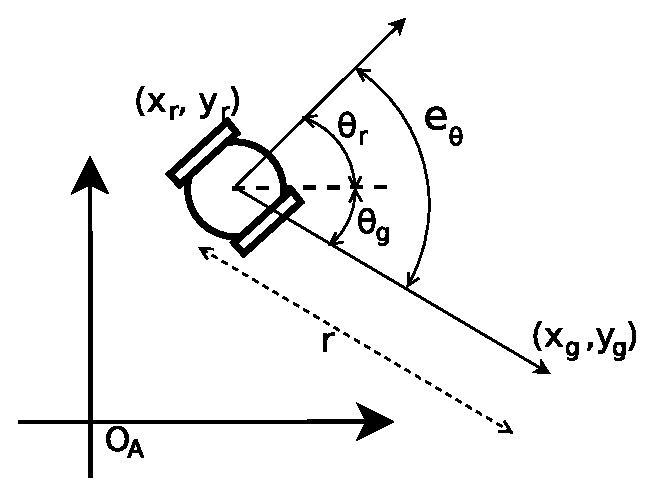
\includegraphics[width=0.5\textwidth]{Figures/GoalPose.eps}
\caption{Posición del robot y posición deseada.}
\label{fig:Coords}
\end{figure}

\subsection{Control de posición}
El objetivo del control es diseñar las señales $v_l$ y $v_r$ de modo que se garantice que el robot llegue a la posición $\left(x_g, y_g\right)$ aun en presencia de incertidumbres (como las dinámicas no modeladas) y perturbaciones. En esta práctica se implementará un control no lineal para lo cual es necesario definir algunas variables.

Considérese el esquema de la figura \ref{fig:Coords}. El ángulo deseado $\theta_g$ corresponde al ángulo del vector de error de posición $\left[x_g - x_r, y_g - y_r\right]^T$, esto es
\[\theta_g = \atantwo\left(y_g - y_r, x_g - x_r\right)\]
de donde se define el error de ángulo
\begin{equation}
  e_{\theta} = \theta_g - \theta_r = \atantwo\left(y_g - y_r, x_g - x_r\right) - \theta_r \label{eq:AngleError}
\end{equation}
Es importante que $e_{\theta}$, al igual que cualquier otra medida angular, se encuentre siempre en el intervalo $(-\pi, \pi]$. Si la diferencia dada en (\ref{eq:AngleError}) resulta en un ángulo mayor que $\pi$  o menor que $-\pi$, se debe hacer el ajuste correspondiente para que $e_{\theta} \in (-\pi, \pi]$  y así se asegure el buen funcionamiento de las leyes de control.

El error de distancia $r$ es simplemente la magnitud del vector de error de posición:
\[r= \left[\left(x_g - x_r\right) + \left(y_g - y_r\right)\right]^{1/2}\]

% En la primera ley de control las velocidades se calculan tomando en cuenta tanto el error de posición como el de ángulo:
%\begin{eqnarray}
%v_{l} &=& -k_{\theta}e_{\theta} + k_d r e^{-\psi e_{\theta}^2}\label{eq:Control11}\\
%v_{r} &=&  k_{\theta}e_{\theta} + k_d r e^{-\psi e_{\theta}^2}\label{eq:Control12}
%\end{eqnarray}
%Nótese que los primeros términos tienen igual magnitud pero signo opuesto, lo que provoca una velocidad angular que es proporcional al error de ángulo. Los segundos términos, al tener el mismo signo y misma magnitud, provocan una velocidad lineal que es proporcional al error de distancia, es decir, el robot se irá deteniendo conforme se acerque al punto meta. La exponencial sirve para hacer pequeña la velocidad lineal cuando el error de ángulo es grande, es decir, este término logra que el robot comience a avanzar hasta que esté apuntando en la dirección correcta.

%En esta ley de control se tienen tres parámetros de diseño: $k_{\theta}>0$, $k_d>0$ y $\psi>0$. Las dos primeras determinan la rapidez con que el robot girará y avanzará hacia el punto meta. La tercera es muy importante. Un valor de $\psi$ muy grande hará que la velocidad lineal decrezca muy rápido cuando crece el error de ángulo, es decir, el robot comenzará a avanzar hasta que esté apuntando casi sin error hacia la meta. Por el contrario, una $\psi$ muy pequeña hará que el robot describa curvas muy grandes.  

Si se considera un robot diferencial cuyo modelo está dado por (\ref{eq:Kinematic1})-(\ref{eq:Kinematic3}), entonces la ley de control dada por 
\begin{eqnarray} 
v_{l} &=& v_{max}e^{-\frac{e_{\theta}^{2}}{\alpha}} + 
\frac{L}{2}\omega_{max}\left(\frac{2}{1+e^{-\frac{e_{\theta}}{\beta}}}-1\right)\label{eq:Control21}\\
v_{r} &=& v_{max}e^{-\frac{e_{\theta}^{2}}{\alpha}} -
\frac{L}{2}\omega_{max}\left(\frac{2}{1+e^{-\frac{e_{\theta}}{\beta}}}-1\right)\label{eq:Control22}
\end{eqnarray}
asegura que el robot alcance la posición deseada $\left(x_g, y_g\right)^T$. Estas ecuaciones también se pueden escribir en términos de las velocidades lineal y angular del robot dadas por:
\begin{eqnarray*}
  v      &=& v_{max}e^{-\frac{e_{\theta}^{2}}{\alpha}}\\
  \omega &=& \omega_{max}\left(\frac{2}{1+e^{-\frac{e_{\theta}}{\beta}}}-1\right)
\end{eqnarray*}

  En la ley de control (\ref{eq:Control21})-(\ref{eq:Control22}) se tienen cuatro parámetros de diseño. $v_{max}$ y $\omega_{max}$ son las velocidades lineales y angulares máximas respectivamente que el robot alcanzará durante su movimiento. Estos parámetros, en principio,  se pueden fijar arbitrariamente, sin embargo, al implementarse en un robot real, deberán ser congruentes con las capacidades de los actuadores del robot.

  Para comprender mejor el funcionamiento de las constantes $\alpha$ y $\beta$, considérese la figura \ref{fig:LinearAndAngular}. 

  \begin{figure}
    \centering
    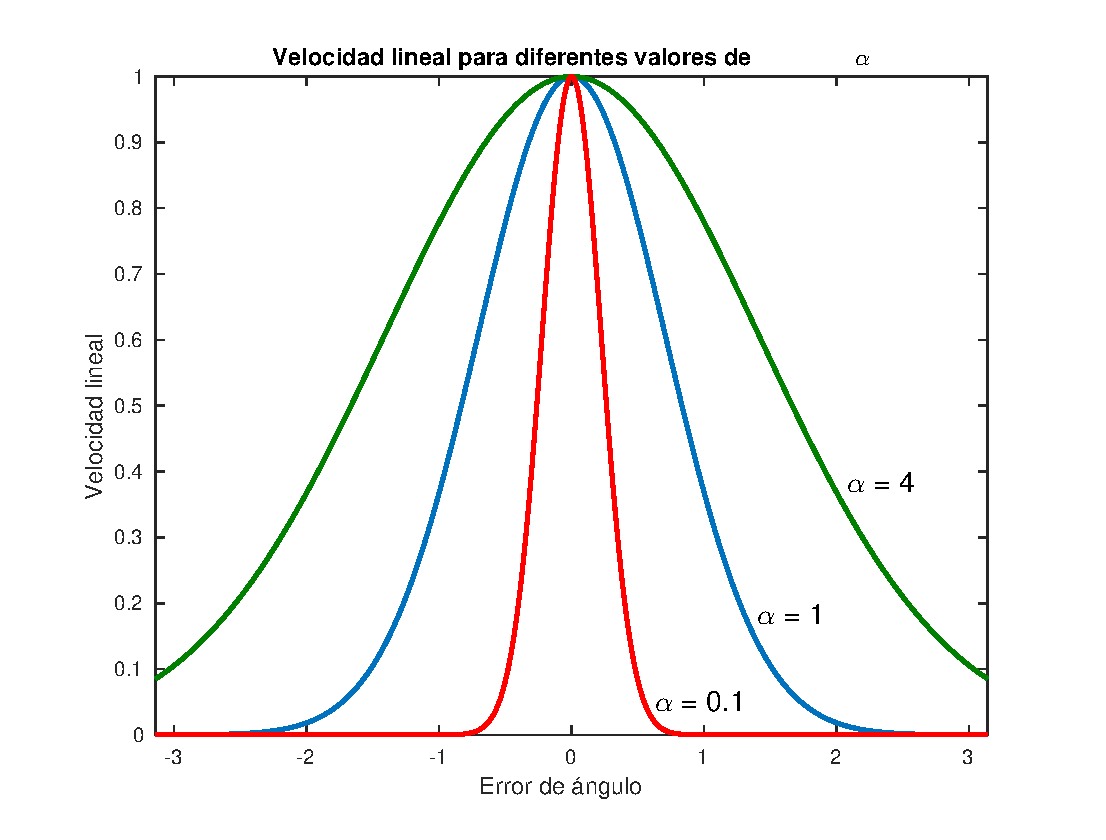
\includegraphics[width=0.45\textwidth]{Figures/LinearSpeed.eps}
    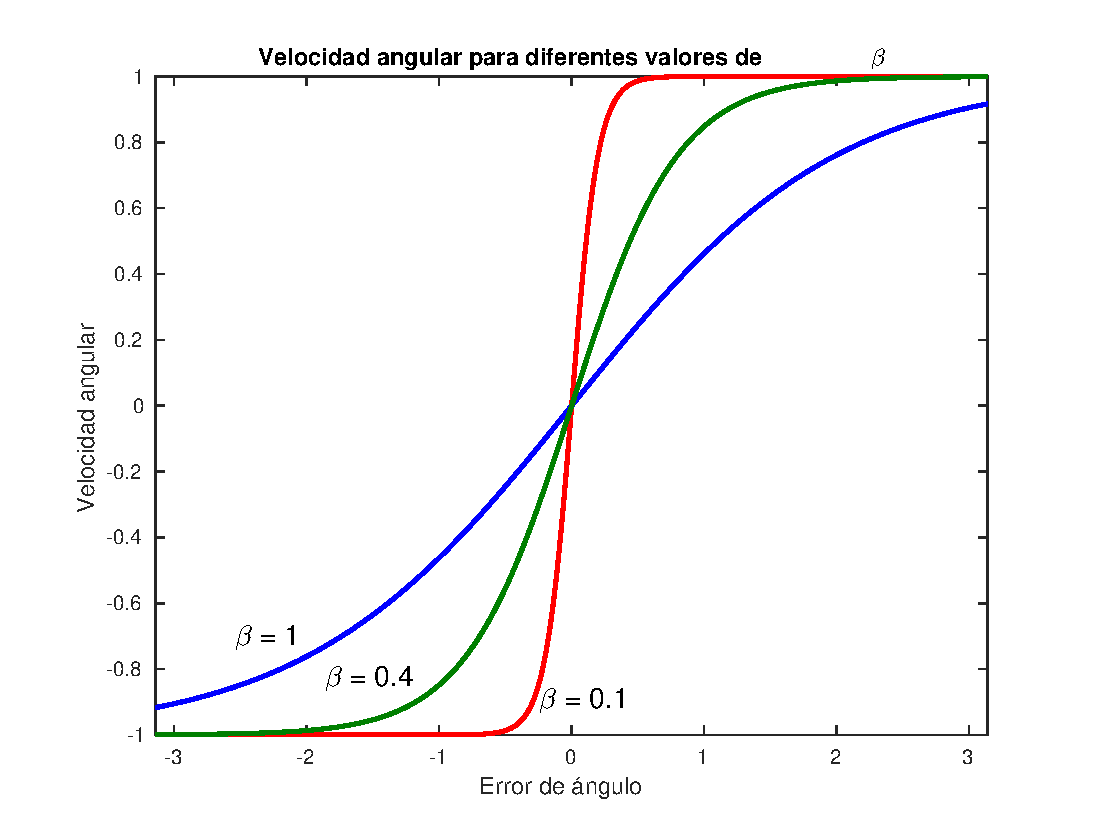
\includegraphics[width=0.45\textwidth]{Figures/AngularSpeed.eps}
    \caption{Velocidades lineal y angular para diferentes parámetros $\alpha$ y $\beta$}
    \label{fig:LinearAndAngular}
  \end{figure}

  Como se puede observar, la constante $\alpha$ determina qué tan rápido decrece la velocidad lineal $v$ cuando el error de ángulo aumenta. Un $\alpha$ muy pequeña hará que la velocidad decrezca rápidamente, esto es, el robot no avanzará hasta que esté ``apuntando directamente'' hacia el punto meta. En otras palabras, primero girará hasta que el error de ángulo sea muy pequeño y hasta entonces avanzará.

  La constante $\beta$ determina qué tan rápido crece la velocidad angular cuando crece el error de ángulo. En general, una $\beta$  pequeña hará que el robot se mantenga siempre ``apuntando'' hacia el punto meta, es decir, ayudará a seguir mejor una ruta deteminada, sin embargo, si $\beta$  es demasiado pequeña, puede generar oscilaciones. 

  
La ley de control (\ref{eq:Control21})-(\ref{eq:Control22} tiene la desventaja de que sólo depende del error de ángulo, es decir, que el robot no disminuye su velocidad conforme se acerca al punto meta. Esto provocará que el robot presente fuertes oscilaciones cuando se encuentre en una región pequeña alrededor del punto meta.

Hay dos formas de abordar este problema. La más sencilla consiste en ejecutar la ley de control sólo si la distancia $r=\sqrt{(x_g - x_r)^2 + (y_g - y_r)^2}$ es mayor que una tolerancia $\epsilon$, es decir:

\[
  \left[\begin{tabular}{c}$v_l$ \\ $v_r$ \end{tabular}\right] =
  \begin{cases}
    \left[
    \begin{tabular}{c}
      $v + \frac{L}{2}\omega$ \\
      $v - \frac{D}{2}\omega$
    \end{tabular}
  \right] \qquad \textrm{si} \qquad \sqrt{(x_g - x_r)^2 + (y_g - y_r)^2} > \epsilon \\
  \\
  \left[
    \begin{tabular}{c}$0$\\$0$\end{tabular}
  \right]  \qquad\qquad \textrm{en otro caso}
  \end{cases}
\]

En este caso, el robot se detendrá bruscamente cuando la magnitud del error de posición sea menor que $\epsilon$, lo cual no es deseable, pues el robot debería disminuir su velocidad conforme se acerca al punto meta.

Por otra parte, también es deseable que el robot aumente su velocidad poco a poco al inicio del movimiento, lo cual no está considerado hasta el momento, pues de acuerdo con (\ref{eq:Control21})-(\ref{eq:Control22}), el robot puede tener una velocidad lineal de $v_{max}$ desde el comienzo de su trayectoria.

\subsection{Máquina de estados}
Una forma sencilla de lograr que el robot acelere y desacelere lentamente es mediante una máquina de estados finita aumentada (AFSM por sus siglas en inglés) que vaya estableciendo el valor $v_{max}$ de la ley de control (\ref{eq:Control21})-(\ref{eq:Control22}). Sea $v_{sm}$ la nueva velocidad máxima, de modo que
\begin{eqnarray}
  v      &=& v_{sm}e^{-\frac{e_{\theta}^{2}}{\alpha}}\label{eq:NewControl1}\\
  \omega &=& \omega_{max}\left(\frac{2}{1+e^{-\frac{e_{\theta}}{\beta}}}-1\right)\label{eq:NewControl2}
\end{eqnarray}
y
\begin{eqnarray*}
  v_l &=& v + \frac{L}{2}\omega\\
  v_r &=& v - \frac{L}{2}\omega
\end{eqnarray*}

El control dado por (\ref{eq:NewControl1})-(\ref{eq:NewControl2}) sirve para alcanzar un punto meta $(x_g, y_g)$, sin embargo lo que se desea es seguir una ruta dada por un conjunto de $N$ puntos $(x^p_i, y^p_i)\quad i\in[0, N-1]$. Para seguir esta ruta basta con fijar como punto meta al punto $(x^p_i, y^p_i)$ que se encuentre ``frente al robot'', es decir, aquel punto de la ruta que esté a una distancia pequeña de la posición actual del robot. ``Distancia pequeña'' puede ser entre 20 [cm] y 50 [cm]. 

La figura \ref{fig:AFSM} muestra los pasos para determinar $v_{sm}$ y el punto meta. En general, $v_{sm}$ se incrementa poco a poco hasta alcanzar el valor de $v_{max}$ y comienza a decrementarse cuando el robot está ``cerca'' del último punto de la ruta deseada, es decir, cuando la distancia $r$ es menor que una constante $r_d$. Cuando el robot está a menos de 30 [cm] del punto meta, éste se cambia por el siguiente punto de la ruta. Los valores de $r_d$ y $\Delta v$ se determinan dependiendo de qué tan rápido el robot debe acelerar y desacelerar. 

\begin{figure}[!h]
  \centering
  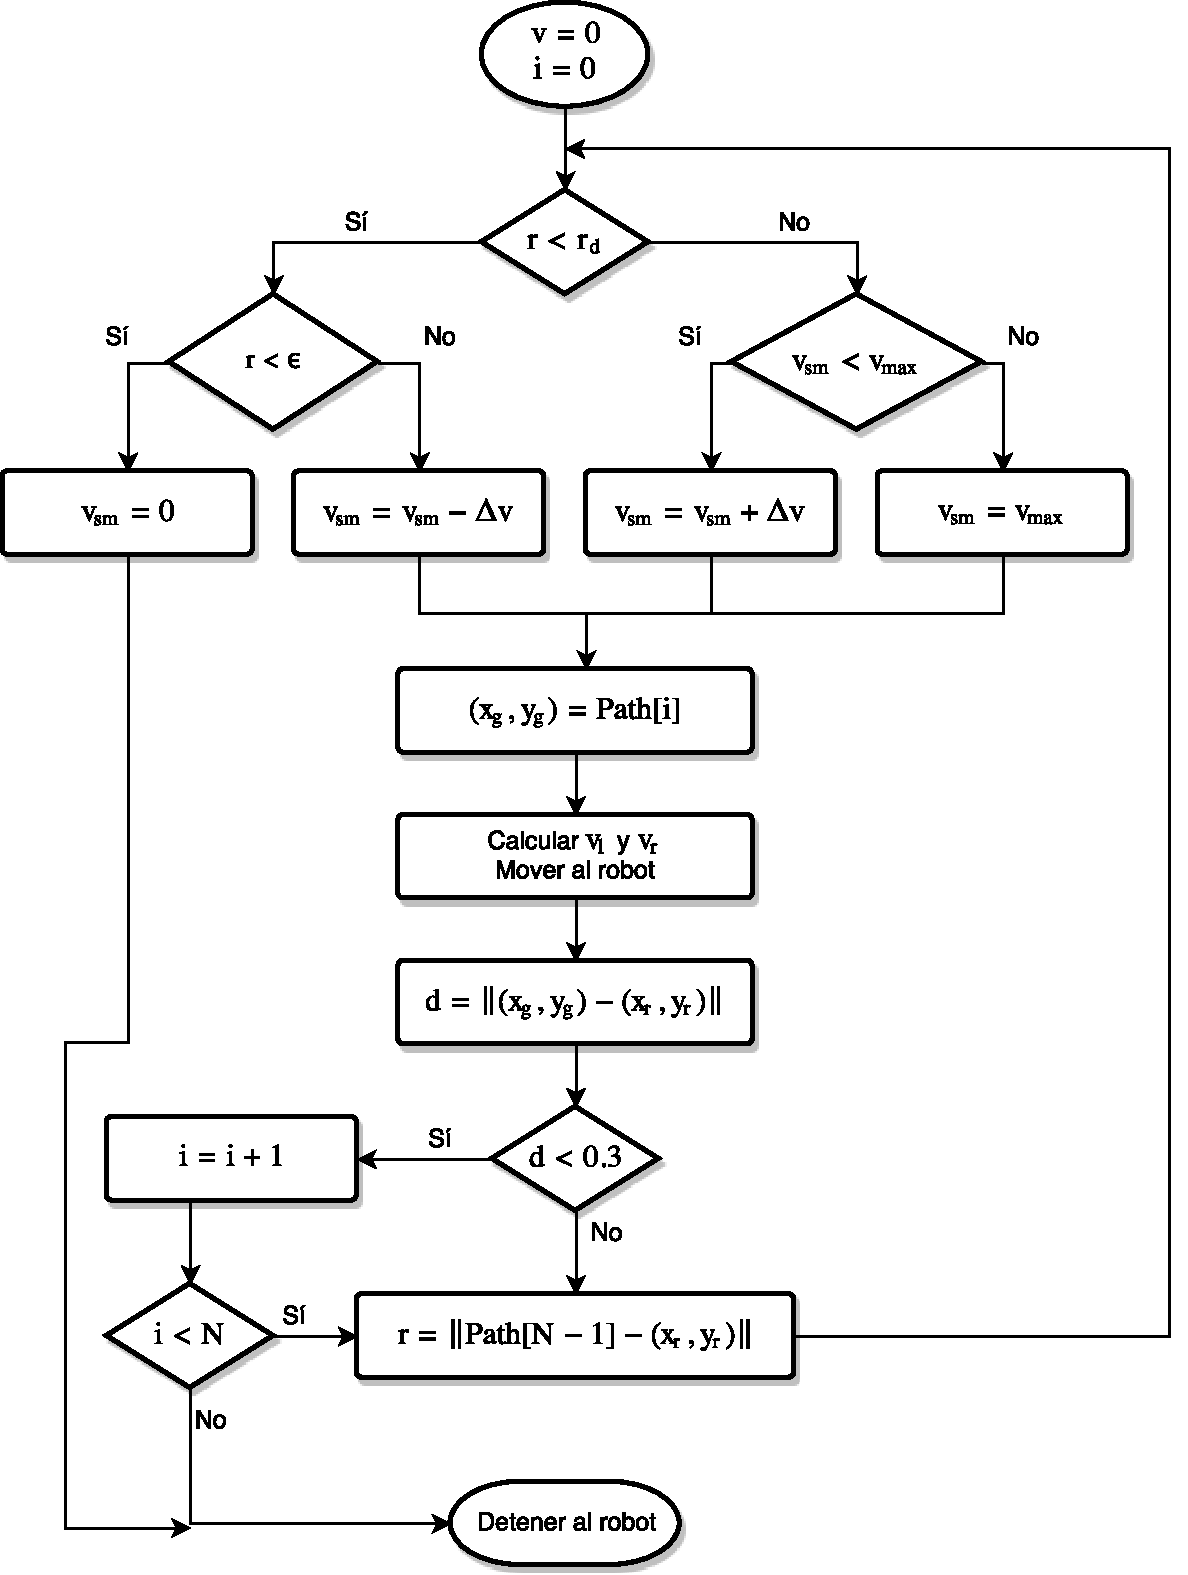
\includegraphics[width=0.7\textwidth]{Figures/AFSM.pdf}
  \caption{Máquina de estados para generar un perfil de velocidad}
  \label{fig:AFSM}
\end{figure}

\section{Tareas}

\subsection{Prerrequisitos}
Antes de continuar, actualice el repositorio y recompile:
\begin{verbatim}
   $  cd ~/RoboticsCourses
   $  git pull origin master
   $  cd catkin_ws
   $  catkin_make
\end{verbatim}

\subsection{Nodo para el control de bajo nivel}
Escribir un nodo de ROS para que el robot siga la ruta calculada en la práctica 5. El nodo debe tener las siguientes carácterísticas:
\begin{itemize}
\item El nombre del nodo debe ser \texttt{low\_level\_control} y debe estar contenido en un paquete del mismo nombre. 
\item La ruta a seguir se obtiene del tópico \texttt{/hardware/a\_star\_path}. Este tópico es el mismo que publica el nodo \texttt{path\_calculator} realizado en la práctica 5.
\item El robot debe comenzar a moverse hasta que se presione el botón \texttt{Exec Path} de la GUI. Al presionar este botón se publica el tópico \texttt{/navigation/execute\_path} de tipo \texttt{std\_msgs::Empty}, por lo que el nodo debe estar suscrito a este tópico. 
\end{itemize}

\subsection{Pruebas experimentales y en simulación}
Probar el nodo \texttt{low\_level\_control} en simulación. Para ello:
\begin{itemize}
\item Ejecute el comando \texttt{roslaunch bring\_up hardware\_simul.launch}
\item Ejecute el nodo \texttt{path\_calculator} realizado en la pŕactica 5.
\item Ejecute el nodo \texttt{low\_level\_control}
\end{itemize}

Ajuste todos los parámetros necesarios hasta que el robot siga la ruta sin oscilaciones ni movimientos bruscos de ningún tipo. Una vez que se logre esto, pruebe el nodo en el robot real. Para ello:

\begin{itemize}
\item Encienda el robot y conecte el cable USB etiquetado como ``USB\_Main'' a cualquier puerto de la computadora.
\item Ejecute el comando \texttt{roslaunch bring\_up hardware\_justina\_winter.launch}
\item Ejecute el nodo \texttt{path\_calculator} realizado en la pŕactica 5.
\item Ejecute el nodo \texttt{low\_level\_control}
\end{itemize}

\textbf{Importante:} recuerde siempre estar atento al movimiento del robot. Si el robot presenta cualquier comportamiento no deseado, \textbf{presione inmediatemente el botón de paro de emergencia}.

\section{Evaluación}
\begin{itemize}
\item El control se probará con varias rutas. Los puntos meta se elegirán aleatoriamente.
\item Para el cálculo de rutas se empleará el nodo hecho en la práctica 5 y el mapa obtenido en la práctica 3.
\item El movimiento del robot debe ser suave, esto es, no se deben presentar oscilaciones ni cambios bruscos en las velocidades de los motores.
\item El robot debe acelerar al inicio de la ruta y desacelerar al acercarse al final.
\item NO puede haber colisiones con ningún objeto. 
\item Las constantes de las leyes de control deben ser fácilmente modificables. 
\item El código debe estar ordenado.
\item \textbf{Importante: } Si el alumno no conoce su código, NO se contará la práctica.
\end{itemize}

\end{document}